\documentclass{beamer}
\usepackage{tikz} %for mindmap
\usetikzlibrary{mindmap} %for mindmap
\usepackage{pgfpages}
\usepackage[backend=bibtex]{biblatex}
\usepackage{multicol}
\usepackage{textpos}
\setbeameroption{hide notes} % Only slides
%\setbeameroption{show only notes} % Only notes
%\setbeameroption{show notes on second screen=right} % Both
\bibliography{../../papers/references.bib}
%\setbeamerfont{footnote}{size=\small}
%\AtEveryCitekey{\clearfield{title}}
%\expandafter\def\expandafter\insertshorttitle\expandafter{%
%   \insertshorttitle\hfill%
%   \insertframenumber\,/\,\inserttotalframenumber}

%
% Choose how your presentation looks.
%
% For more themes, color themes and font themes, see:
% http://deic.uab.es/~iblanes/beamer_gallery/index_by_theme.html
%
\mode<presentation>
{
%   \usetheme{Warsaw}      % or try Darmstadt, Madrid, Warsaw, ...
   \usetheme{Frankfurt}      % or try Darmstadt, Madrid, Warsaw, ...
   \usecolortheme{default} % or try albatross, beaver, crane, ...
   \usefonttheme{default}  % or try serif, structurebold, ...
   \setbeamertemplate{navigation symbols}{}
%   \setbeamertemplate{caption}[numbered]
%   \setbeamertemplate{footline}[frame number]
%   \usepackage{appendixnumberbeamer} %starts slide numbering over after \appendix
} 

\usepackage[english]{babel}
%\usepackage[utf8x]{inputenc} %Doesn't play well with biblatex
\usepackage{amssymb}
\usepackage{bm}
\usepackage{color}
\usepackage{graphicx}

\newcommand{\red}[1]{{\color{red}{#1}}}
\newcommand{\ket}[1]{\left| #1 \right>}
\newcommand{\bra}[1]{\left< #1 \right|}
\newcommand{\braket}[2]{\left< #1 | #2 \right>}
\newcommand{\ketbra}[2]{\left| #1 \right> \left< #2 \right|}
\newcommand{\expect}[1]{\left< #1 \right>}
\newcommand{\fpij}{f_p(r_{ij})}
\newcommand{\vpij}{v_p(r_{ij})}
\newcommand{\Opij}{\mathcal{O}_{ij}^p}
\newcommand{\fOpij}{\sum\limits_{i<j}\sum\limits_p \fpij\Opij}
\newcommand{\fqkl}{f_q(r_{kl})}
\newcommand{\Oqkl}{\mathcal{O}_{kl}^q}
\newcommand{\fOqkl}{\sum\limits_{k<l}\sum\limits_q \fqkl\Oqkl}
\newcommand{\fOqklip}{\sum\limits_{k<l,\mathrm{ip}}\sum\limits_q \fqkl\Oqkl}
\newcommand{\fOqklquad}{\sum_{\substack{k<l\\ij \ne kl}}\sum\limits_q \fqkl\Oqkl}
\newcommand{\f}[2]{f_{#1}(r_{#2})}
\renewcommand{\O}[2]{\mathcal{O}_{#2}^{#1}}
\newcommand{\fO}[2]{\sum\limits_{#1} f_{#1}(r_{#2})\mathcal{O}_{#2}^{#1}}
\newcommand{\R}{\mathbf{R}}
\newcommand{\dt}{\Delta\tau}
\newcommand{\ti}{\bm{\tau}_i}
\newcommand{\tj}{\bm{\tau}_j}
\newcommand{\si}{\bm{\sigma}_i}
\newcommand{\sj}{\bm{\sigma}_j}
\newcommand{\sfont}{6}
\newcommand{\sspace}{10.2}
\newcommand{\Oijp}{\mathcal{O}^p_{ij}}

\title{Computational Nuclear Physics}
\author{Cody L. Petrie}
\institute{Arizona State University \\ Tempe, AZ}
\date{}

\begin{document}

\begin{frame}
   \titlepage
\end{frame}

\iffalse
\begin{frame}{Outline}
\begin{itemize}
   \item Quantum Monte Carlo methods
   \item Improved trial wave function
   \item Alpha formation in nearly neutron matter - preliminary
   \item Another Improved trial wave function - preliminary
\end{itemize}
\end{frame}
\fi

\begin{frame}{Nuclear Physics}
\begin{itemize}
   \item Pictures of things that nuclear physics is good for, like \ldots
   \begin{itemize}
      \item Nuclear power (on earth, spacecraft, etc.)
      \item Medical imaging
      \item Basic structure of nuclei
      \item Neutron Stars
   \end{itemize}
\end{itemize}
\end{frame}

\begin{frame}{Integrals}
\begin{itemize}
   \item Ground state (lowest) energy
   \begin{equation*}
      E_{gs} = \int \psi^*(\mathbf{R})H\psi(\mathbf{R}) d\mathbf{r_1}d\mathbf{r_2}\ldots d\mathbf{r_N}
   \end{equation*}
   \item<2-> If you know what an integral is, go ahead and panic.
   \item<3-> If you don't know what an integral is, it's easy. Here I'll show you \ldots
\end{itemize}
\end{frame}

\begin{frame}{What is an integral?}
\begin{itemize}
   \item Let's say you wanted to know the length of a line at disneyland. You can have 1 stick of known length. Does a smaller or larger stick make it faster? Which makes it more accurate?
\end{itemize}

\onslide<1>{
\begin{textblock*}{\textwidth}(0.0cm,-0.6cm) % {block width} (coords)
\begin{figure}[h]
   \centering
   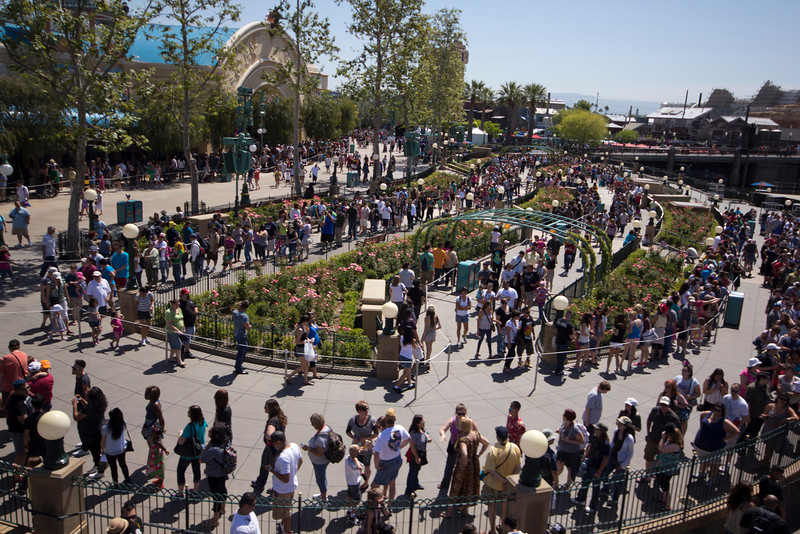
\includegraphics[width=0.5\textwidth]{figures/ariel_openingday.jpg}
\end{figure}
\end{textblock*}
}
\onslide<2->{
\begin{textblock*}{\textwidth}(0.0cm,-0.6cm) % {block width} (coords)
\begin{figure}[h]
   \centering
   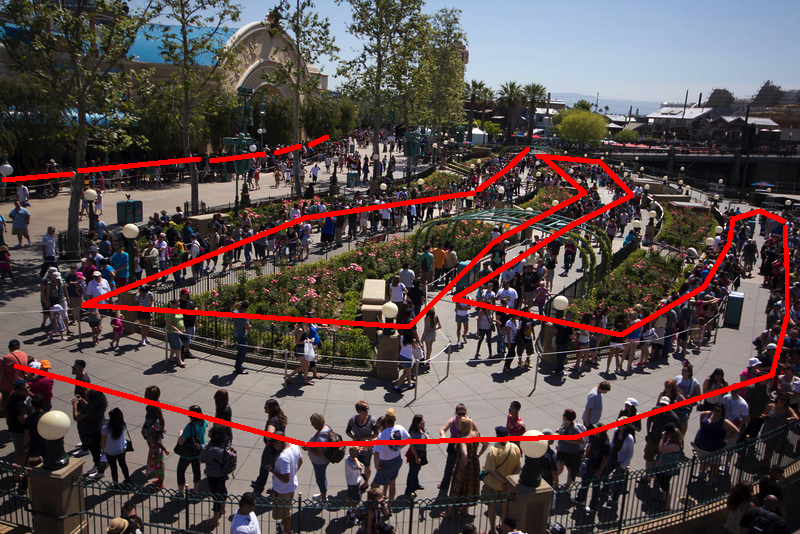
\includegraphics[width=0.5\textwidth]{figures/ariel_openingday_lines.png}
\end{figure}
\end{textblock*}
}
~\\~\\~\\~\\~\\~\\~\\~\\
\uncover<2>{
\begin{equation*}
   L = \sum\limits_i l_i \xrightarrow{l_i\rightarrow 0} \int\limits_\text{line} dl
\end{equation*}
}
\end{frame}

\begin{frame}{Monte Carlo}
\onslide<1>{
\begin{textblock*}{\textwidth}(2.5cm,-0.3cm) % {block width} (coords)
\begin{figure}[h]
   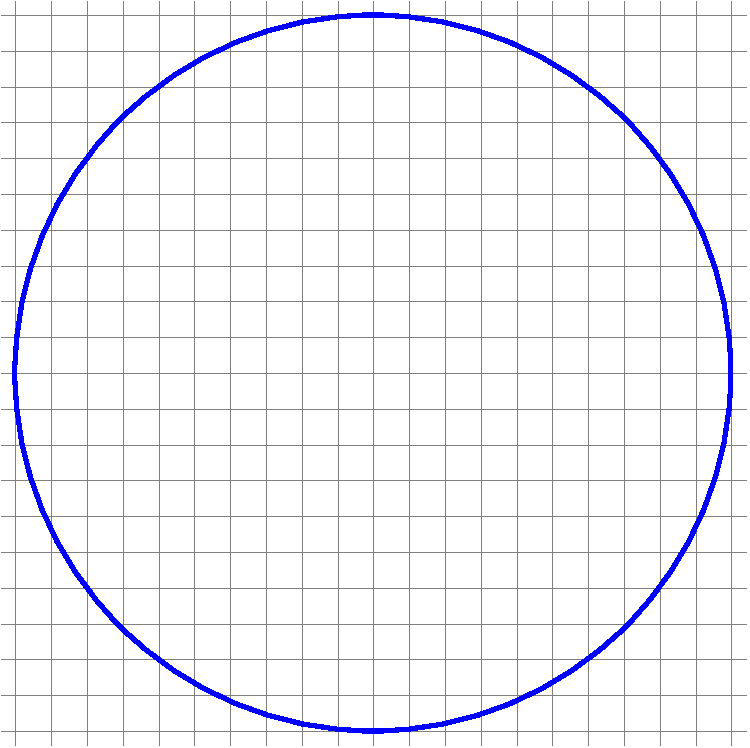
\includegraphics[width=0.4\textwidth]{figures/circle_grid.pdf}
\end{figure}
\end{textblock*}
}
\only<1>{
\vspace{5.5cm}
\begin{equation*}
   A_\text{circle} = \sum\limits_{i}\sum\limits_{j} dx_i dy_j
\end{equation*}
}


\onslide<2>{
\begin{textblock*}{\textwidth}(-3.3cm,1.0cm) % {block width} (coords)
\begin{figure}[h]
   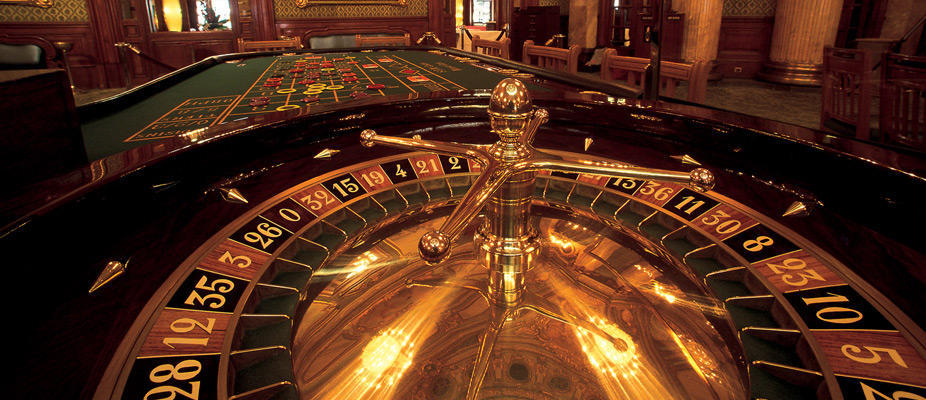
\includegraphics[width=0.4\textwidth]{figures/monte_carlo_casino.jpg}
\end{figure}
\end{textblock*}
\begin{textblock*}{\textwidth}(2.5cm,-0.3cm) % {block width} (coords)
\begin{figure}[h]
   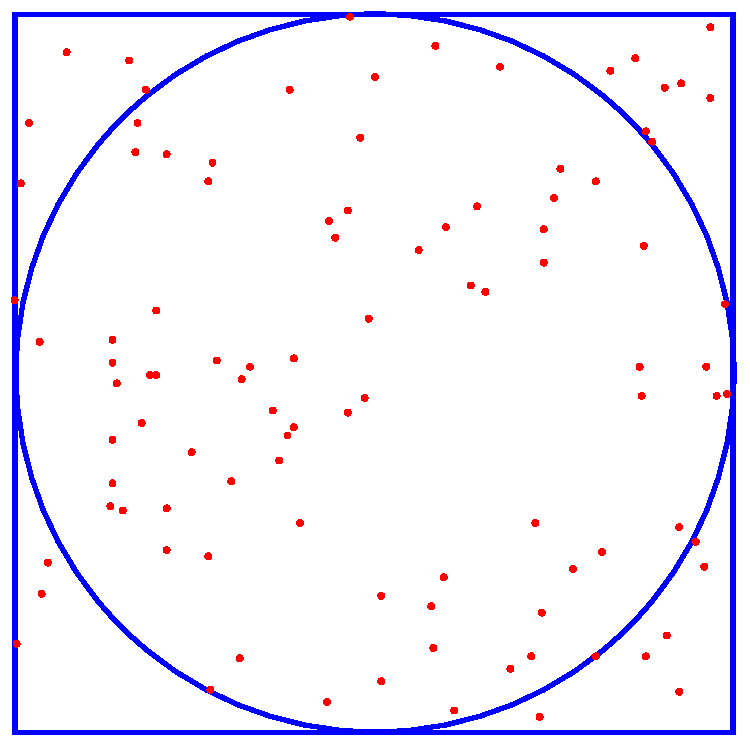
\includegraphics[width=0.4\textwidth]{figures/circle_square_points.pdf}
\end{figure}
\end{textblock*}
}
\vspace{5.5cm}
\only<2>{
\begin{equation*}
   \frac{A_\text{circle}}{A_\text{box}} = \frac{\text{\# points in the circle}}{\text{\# points in the box (total)}}
\end{equation*}
}
\end{frame}

\begin{frame}{Monte Carlo Example}
\begin{itemize}
   \item You can estimate $\pi=3.14159$ using the method above.
\begin{equation*}
   \frac{A_\text{circle}}{A_\text{box}} = \frac{\pi r^2}{(2r)(2r)} = \frac{\pi}{4} = \frac{\text{\# points in the circle}}{\text{\# points in the box (total)}}
\end{equation*}
\begin{equation*}
   \pi=4\frac{\text{\# points in the circle}}{\text{\# points in the box (total)}}
\end{equation*}
\end{itemize}
\begin{figure}[h]
   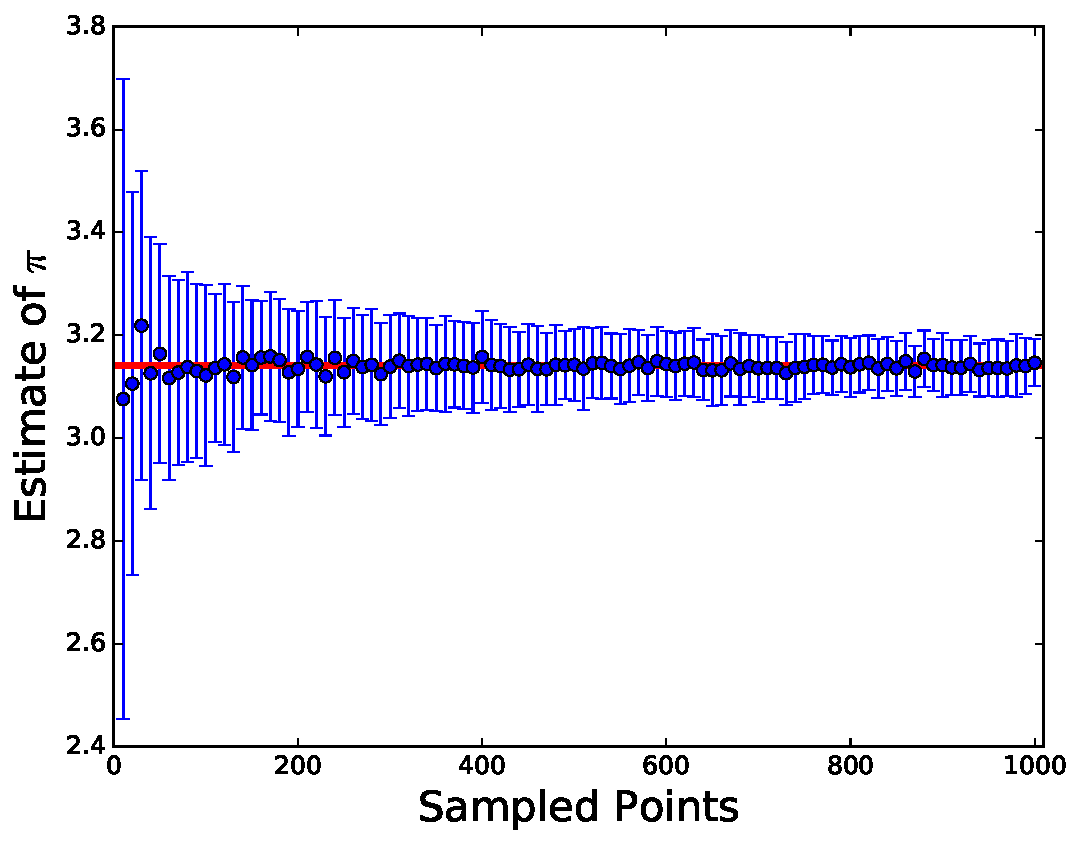
\includegraphics[width=0.55\textwidth]{figures/pi_estimate.pdf}
\end{figure}
\end{frame}

\begin{frame}{Monte Carlo on a Supercomputer}
\begin{textblock*}{\textwidth}(-3.6cm,0.0cm) % {block width} (coords)
\begin{figure}[h]
   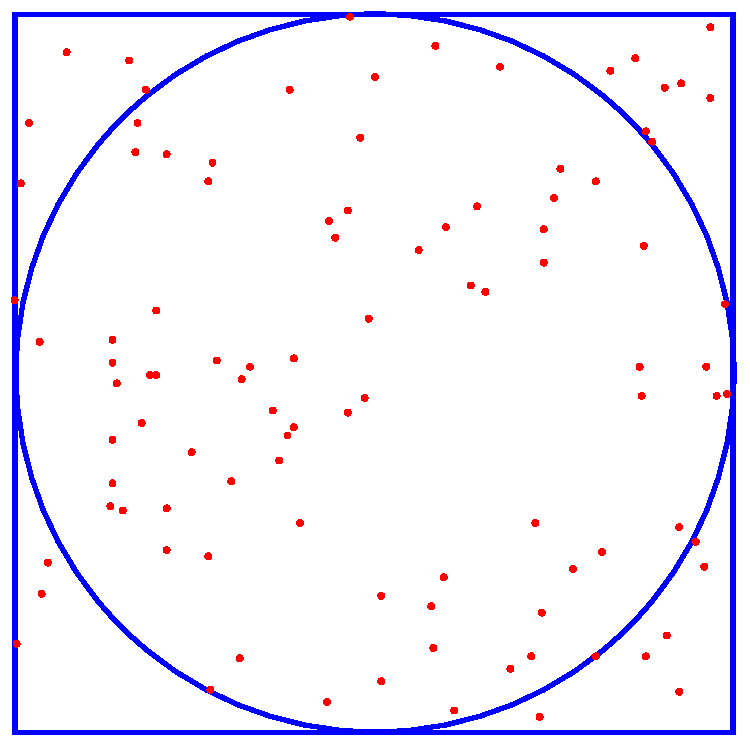
\includegraphics[width=0.3\textwidth]{figures/circle_square_points.pdf}
\end{figure}
\end{textblock*}
\begin{textblock*}{\textwidth}(2.2cm,-0.5cm) % {block width} (coords)
\begin{figure}[h]
   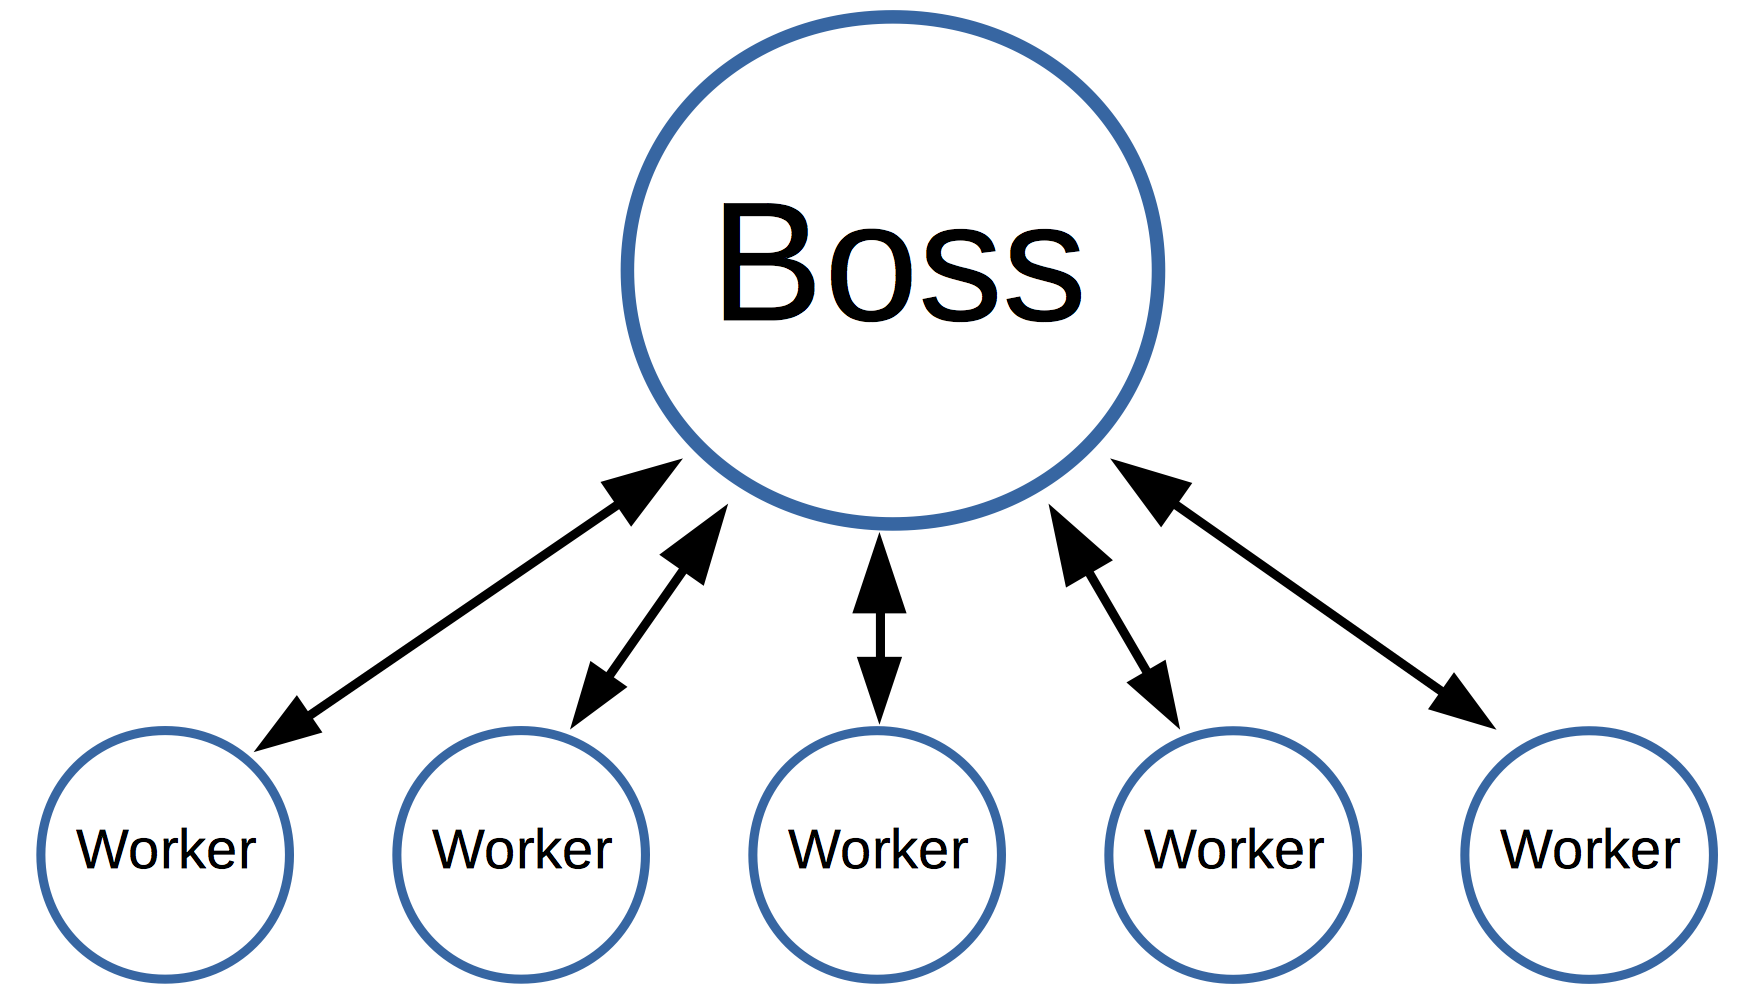
\includegraphics[width=0.7\textwidth]{figures/boss_worker.png}
\end{figure}
\end{textblock*}
\vspace{4.0cm}
\begin{equation*}
   E_{gs} = \int \psi^*(\mathbf{R})H\psi(\mathbf{R}) d\mathbf{r_1}d\mathbf{r_2}\ldots d\mathbf{r_N}
\end{equation*}
\begin{equation*}
   \psi_T^*(\mathbf{R}) H \psi_T(\mathbf{R}) \text{ at each point}
\end{equation*}
\end{frame}

\begin{frame}{Monte Carlo in Nuclear Physics}
\begin{equation*}
   E_{gs} = \int \psi^*(\mathbf{R})H\psi(\mathbf{R}) d\mathbf{r_1}d\mathbf{r_2}\ldots d\mathbf{r_N}
\end{equation*}
\begin{itemize}
   \item Guess $\Psi_T$
   \item Get a good guess for $H$ from somebody else
   \item Put it on a supercomputer
   \item Change $\Psi_T$ until you get the lowest energy you can (Variational Monte Carlo)
\end{itemize}
\end{frame}

\begin{frame}{Better $\Psi_T$ Results}
\begin{textblock*}{\textwidth}(0.0cm,-0.6cm) % {block width} (coords)
\begin{figure}[h]
   \centering
   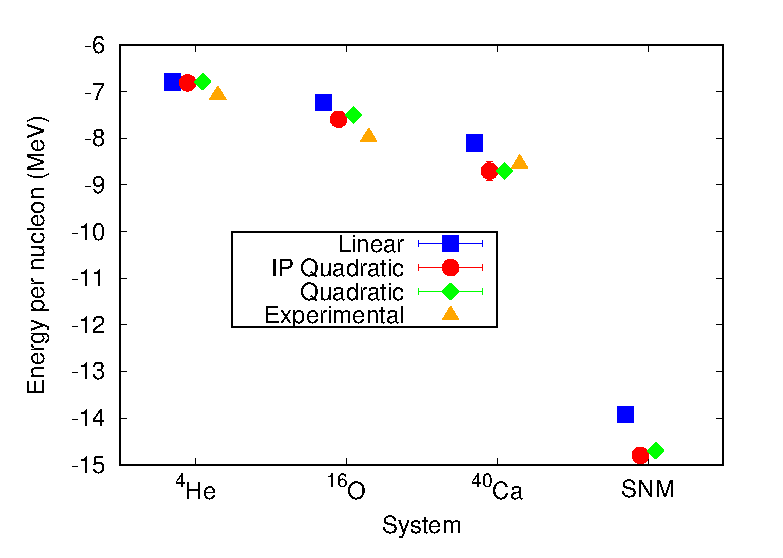
\includegraphics[width=0.6\textwidth]{figures/energy.eps}
\end{figure}
\end{textblock*}
~\\~\\~\\~\\~\\~\\~\\~\\
\tiny
\begin{table}[htb]
\centering
\caption[]{Energy (*per nucleon) in MeV}
\begin{tabular}{ccccc}
\hline\hline
System & Linear & IP Quadratic & Quadratic & Experimental\\
\hline
${}^{4}${He}   & -27.14(4) & -27.22(3)    & -27.11(3)    & -28.295   \\  
${}^{16}${O}   & -115.7(9) & -121.5(1.5)  & -120.0(1.4)  & -127.62   \\  
${}^{40}${Ca}  & -324(3)   & -347(8)      & -349(5)      & -342.1     \\  
SNM*           & -13.92(6) & -14.80(7)    & -14.70(11)   &           \\  
\hline\hline
\end{tabular}
\label{tab:psi2}
\end{table}
{\tiny D. Lonardoni et al. \textit{Phys. Rev. C.,} \textbf{97}, 044318, 2018.}
\end{frame}

\begin{frame}{Better $\Psi_T$ Cost}
\begin{figure}[h]
   \centering
   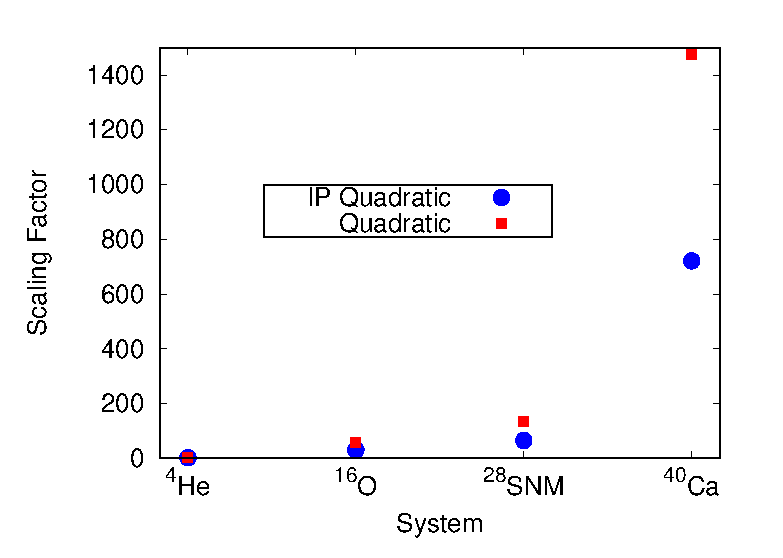
\includegraphics[width=0.65\textwidth]{figures/scaling.eps}
\end{figure}
\vspace{-0.2cm}
\begin{table}[h!]
   \centering
   \begin{tabular}{ccccc}
      \hline \hline
       & $^{4}$He & $^{16}$O & SNM(28) & $^{40}$Ca \\
      \hline
      IP Quadratic & 1.73 & 30.7 & 64.8 & 720.9 \\
      Quadratic & 2.00 & 58.8 & 133.6 & 1473.9 \\
      \hline \hline
   \end{tabular}
\end{table}
\end{frame}

\begin{frame}{$^4$He Nuclei Forming in Neutron Stars}
\begin{itemize}
   \item Use new wave function to study $\alpha$ formation in the inner crust of neutron stars.
   \begin{equation*}
      E_\alpha = E_\text{Nn+2p} - E_\text{(N-2)n}
   \end{equation*}
\end{itemize}
\vspace{-0.5cm}
\begin{figure}[h]
   \centering
   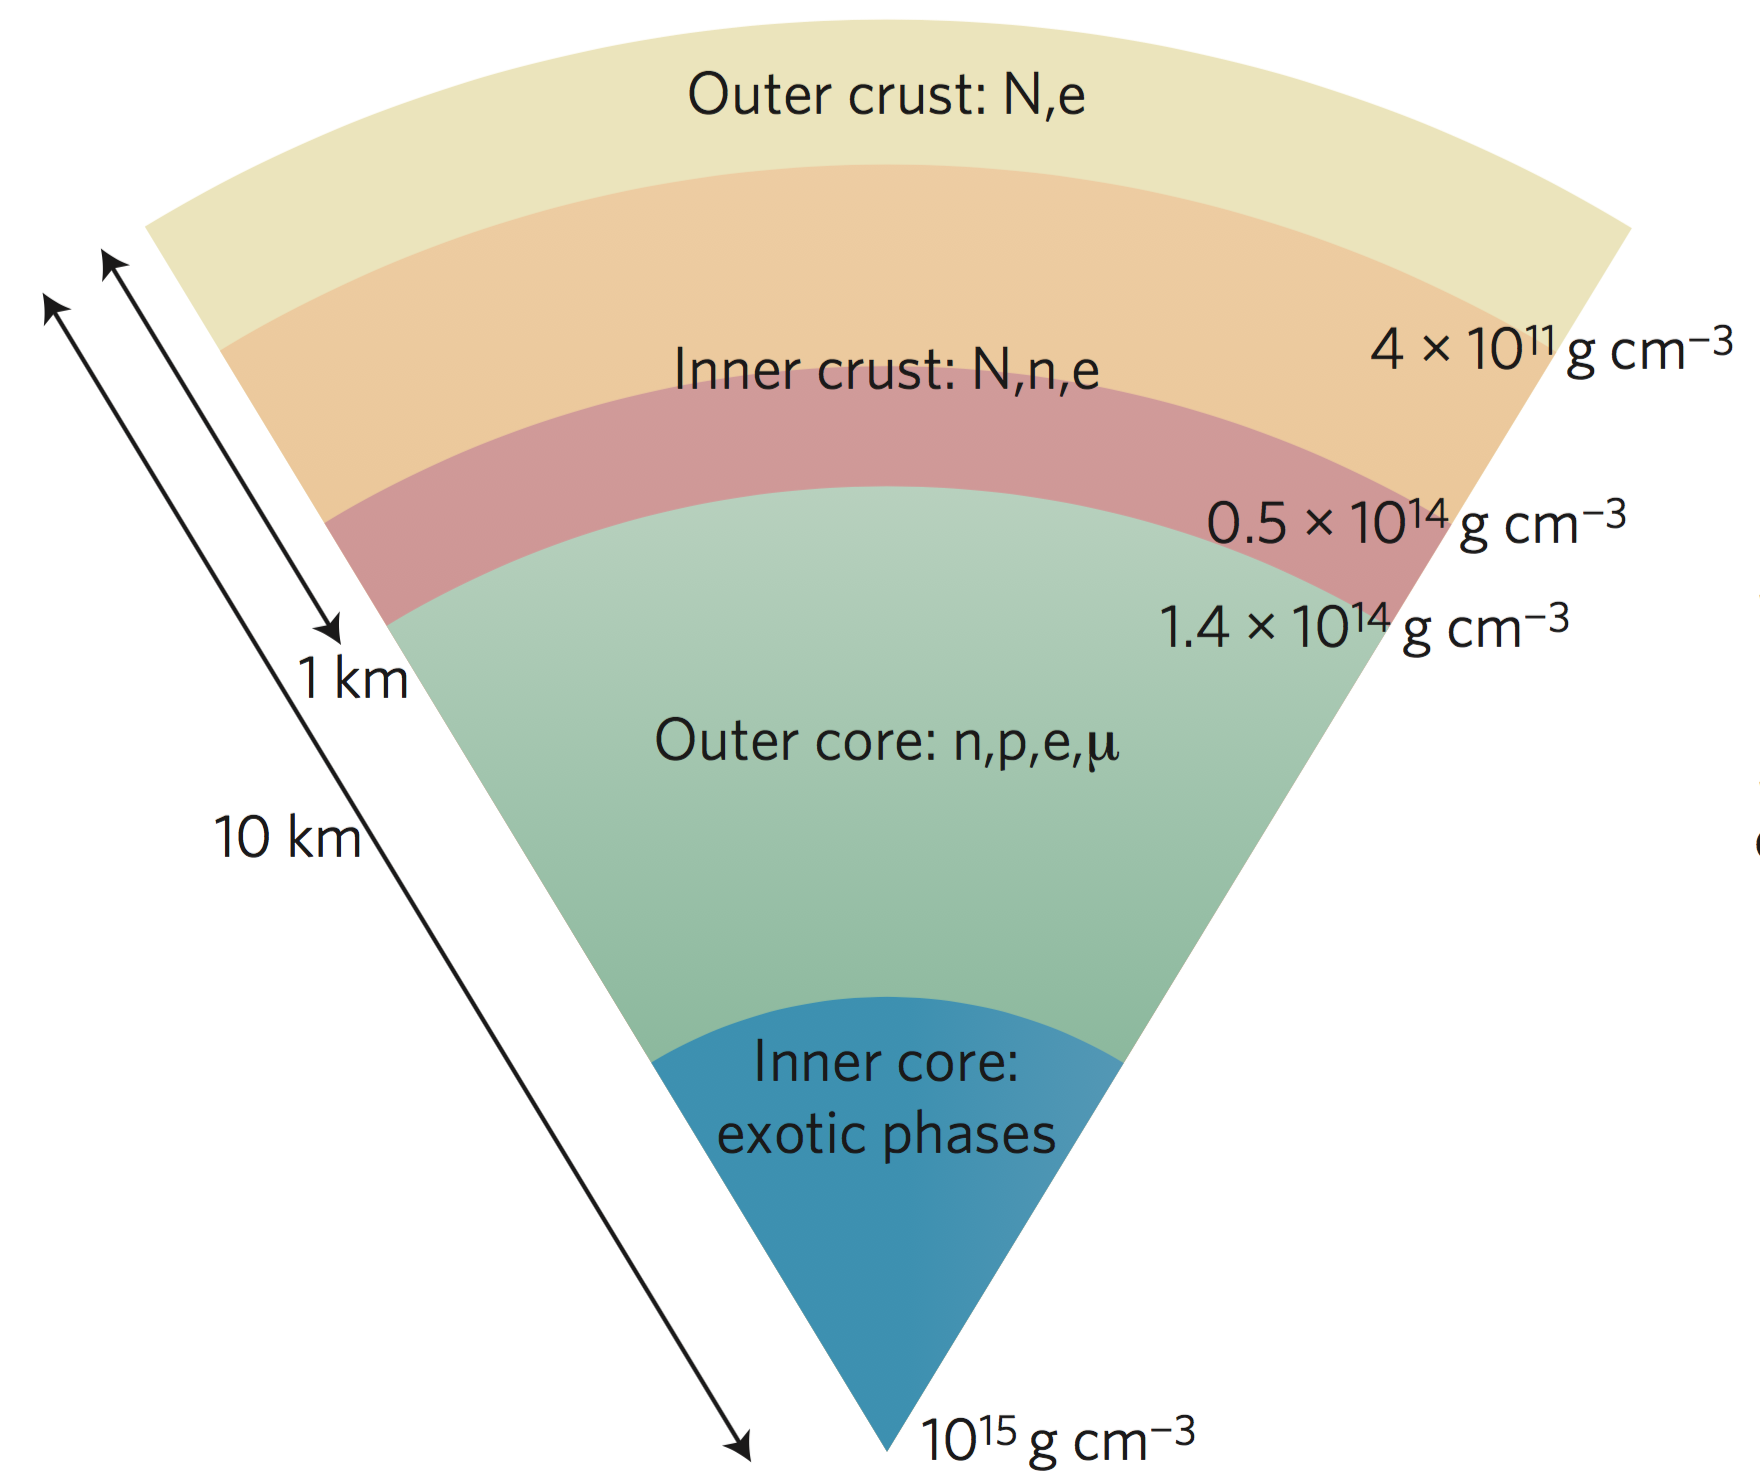
\includegraphics[width=0.5\textwidth]{figures/neutronstar.png}
\end{figure}
W. Newton {\it Nature Physics} {\bf 9}, 396-397 (2013)
%\begin{textblock*}{\textwidth}(8.1cm,-4.6cm) % {block width} (coords)
\begin{textblock*}{\textwidth}(8.1cm,-4.5cm) % {block width} (coords)
   \tiny $\approx$ 0.00024 fm$^{-3}$
\end{textblock*}
%\begin{textblock*}{\textwidth}(7.8cm,-4.1cm) % {block width} (coords)
\begin{textblock*}{\textwidth}(7.8cm,-4.0cm) % {block width} (coords)
   \tiny $\approx$ 0.030 fm$^{-3}$
\end{textblock*}
%\begin{textblock*}{\textwidth}(7.6cm,-3.8cm) % {block width} (coords)
\begin{textblock*}{\textwidth}(7.6cm,-3.7cm) % {block width} (coords)
   \tiny $\approx$ 0.084 fm$^{-3}$
\end{textblock*}
%\begin{textblock*}{\textwidth}(6.4cm,-1.3cm) % {block width} (coords)
\begin{textblock*}{\textwidth}(6.4cm,-1.2cm) % {block width} (coords)
   \tiny $\approx$ 0.60 fm$^{-3}$
\end{textblock*}
\end{frame}

\begin{frame}{\large Alpha Particle Clustering in Mostly Neutron Matter}
\begin{itemize}
   \item If alpha particles form in nearly neutron matter then we should be able to estimate their energy by
   \begin{equation*}
      E_\alpha = E_\text{14n+2p} - E_\text{12n}
   \end{equation*}
   \item Both energies decreased, but the combination did not always.
   \vspace{-0.25cm}
   \begin{columns}
   \begin{column}{0.5\textwidth}
   \begin{figure}[h]
      \centering
      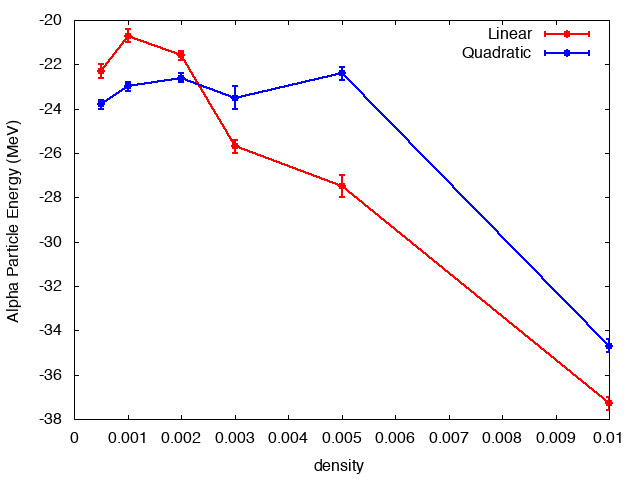
\includegraphics[width=\textwidth]{figures/clusterplot.png}
   \end{figure}
   \end{column}
   \begin{column}{0.5\textwidth}
   \begin{table}[h!]
      \centering
      \caption{Alpha energy in MeV}
      \begin{tabular}{ccc}
         \hline \hline
         $\rho$ (fm$^{-3}$) & lin & ip \\
         \hline
         0.0005& -22.3(3)  & -23.8(2)  \\
         0.001 & -20.7(3)  & -23.0(2)  \\
         0.002 & -21.6(2)  & -22.6(2)  \\
         0.003 & -25.7(3)  & -23.5(5)  \\
         0.005 & -27.5(5)  & -22.4(3)  \\
         0.01  & -37.3(3)  & -34.7(3)  \\
         \hline \hline
      \end{tabular}
   \end{table}
   \end{column}
   \end{columns}
\end{itemize}
\end{frame}

\begin{frame}{Picture References}
\tiny
\textbf{Ariel line on opening day (accessed 4 Aug 2018):} \url{https://forums.wdwmagic.com/threads/omg-little-mermaid-is-sucha-failure.753509/page-2} \\
\textbf{Monte Carlo casino (accessed 6 Aug 2018):} \url{http://www.montecarlosbm.com/luxury-casinos-monaco-3/monte-carlo-casino/}
\end{frame}

\end{document}
